% =============================================================================
%  Section 3.2 — Thiết kế tầng tri thức
%  Subsections:
%    3.2.1  Ontology Chèo - nền tảng tri thức
%    3.2.2  Chuyển đổi và mở rộng lược đồ
%    3.2.3  Cơ chế hỗ trợ truy xuất
%    3.2.4  Danh mục thực thể
% =============================================================================

\section{Thiết kế tầng tri thức}
\label{sec:knowledge_design}

\subsection{Ontology Chèo - nền tảng tri thức}
\label{sec:ontology_cheo}

Hệ thống GraphRAG được đề xuất kế thừa ontology về nghệ thuật Chèo xây dựng trong khóa luận tốt nghiệp của chị Trương Quỳnh Giang~\cite{Giang2025}. Ontology được hình thức hoá theo chuẩn OWL, là cơ sở lý thuyết phù hợp để xây dựng nên đồ thị tri thức phục vụ cho hệ thống truy xuất thông tin.

\textbf{Kiến trúc.}
Ontology tổ chức tri thức theo mô hình phân lớp với 7 lớp, 7 thuộc tính quan hệ (object properties) và 27 thuộc tính dữ liệu (data properties), với chi tiết từng lớp cùng vai trò ngữ nghĩa và tập thuộc tính dữ liệu tương ứng (Bảng~\ref{tab:ontology_classes}).

\begin{table}[ht!]
  \centering
  \caption{Bảy lớp trong Chèo Ontology và các thuộc tính dữ liệu tương ứng.}
  \label{tab:ontology_classes}
  \renewcommand{\arraystretch}{1.35}
  \small
  \begin{tabular}{p{3.5cm} p{3.3cm} p{7.99cm}}
    \toprule
    \textbf{Lớp} & \textbf{Vai trò} & \textbf{Thuộc tính dữ liệu} \\
    \midrule
    \texttt{Play}
      & Vở chèo
      & \texttt{title}, \texttt{summary}, \texttt{author}, \texttt{sceneNumber} \\[2pt]
    \texttt{Character}
      & Nhân vật trong vở
      & \texttt{charName}, \texttt{description}, \texttt{mainType}, \texttt{subType}, \texttt{charGender} \\[2pt]
    \texttt{Actor}
      & Diễn viên
      & \texttt{actorName}, \texttt{actorGender} \\[2pt]
    \texttt{Scene}
      & Trích đoạn
      & \texttt{sceneName}, \texttt{sceneSummary}, \texttt{versionNumber} \\[2pt]
    \texttt{Version}
      & Phiên bản biểu diễn
      & \texttt{showDate}, \texttt{vidVersion}, \texttt{videoDuration}, \texttt{resolution},
        \texttt{aspectRatio}, \texttt{startTime}, \texttt{endTime}, \texttt{ID} \\[2pt]
    \texttt{RoleAssignment}
      &  Phân công vai diễn
      & - \\[2pt]
    \texttt{Appearance}
      & Một lần xuất hiện trong video
      & \texttt{start}, \texttt{end}, \texttt{emotion}, \texttt{subtitle}, \texttt{ED} \\
    \bottomrule
  \end{tabular}
\end{table}

Bảy thuộc tính quan hệ tạo thành cấu trúc liên kết giữa các thực thể trong đồ thị: lớp Play kết nối tới Character và Scene qua \texttt{HAS\_CHARACTER} và \texttt{HAS\_SCENE}; Scene kết nối tới Version qua \texttt{HAS\_VERSION}. Lớp trung gian \texttt{RoleAssignment} kết nối ra ba hướng qua \texttt{PERFORMED\_BY}~(Actor), \texttt{FOR\_CHARACTER}~(Character) và \texttt{IN\_VERSION}~(Version), đồng thời nối sang Appearance qua \texttt{HAS\_APPEARANCE}.

\textbf{Độ phủ tri thức.}
Ontology bao quát \textbf{bảy vở chèo} kinh điển trong kho lưu trữ của Trường Đại học Sân khấu – Điện ảnh Hà Nội: Quan Âm Thị Kính, Kim Nham, Trương Viên, Lưu Bình Dương Lễ, Chu Mãi Thần, Từ Thức và Trịnh Nguyên. Tổng cộng \textbf{400 thực thể} (individuals) được định nghĩa tường minh, gồm 7 vở diễn, 38 nhân vật, 41 diễn viên, 15 trích đoạn, 27 phiên bản biểu diễn, 76 phân công vai diễn và 196 Appearance. Mỗi Appearance ghi nhận một lần xuất hiện của vai diễn trong video kèm thời điểm bắt đầu, thời điểm kết thúc, cảm xúc và lời thoại. Toàn bộ thực thể được xây dựng từ dữ liệu thực tế của nhà trường, đảm bảo tính xác thực của cơ sở tri thức.

\textbf{Cơ sở kế thừa.}
Ontology này đáp ứng ba tiêu chí nền tảng để trở thành nguồn tri thức đáng tin cậy cho hệ thống GraphRAG: (i) \textit{tính nhất quán logic} (cấu trúc OWL với ràng buộc domain/range trên từng object property cho phép bộ suy luận của cơ sở dữ liệu tự động phát hiện mâu thuẫn ngữ nghĩa khi lưu trữ), (ii) \textit{khả năng mô hình hoá miền tri thức} (các lớp trung gian \texttt{RoleAssignment} và \texttt{Appearance} biểu diễn được quan hệ ba-ngôi giữa diễn viên–nhân vật–phiên bản trình diễn mà các mô hình đơn giản không nắm bắt được) và (iii) \textit{chiều sâu dữ liệu} (thông tin được lưu trữ trọn vẹn, với nhiều thuộc tính dữ liệu chi tiết cho phép phân tích vượt ngoài truy xuất thực thể đơn thuần).

Tuy nhiên, khi đặt trong bối cảnh hỏi-đáp thời gian thực, mô hình OWL thuần tuý bộc lộ hai hạn chế kỹ thuật: (i) \textit{chi phí suy luận cao} -- truy vấn đa bước và suy luận quan hệ gián tiếp qua bộ suy luận ontology có chi phí tính toán lớn, không khả thi tại thời điểm truy vấn; và (ii)\textit{ thiếu hỗ trợ tìm kiếm văn bản} -- truy vấn theo thuộc tính chuỗi (đặc biệt với tên riêng tiếng Việt có nhiều biến thể) không được tối ưu sẵn, không có cơ chế khớp không phân biệt hoa-thường hay khớp gần đúng. Hai hạn chế này dẫn đến quyết định chuyển đổi sang mô hình property graph nhằm đảm bảo hiệu năng truy xuất mà vẫn duy trì cấu trúc ngữ nghĩa của ontology ban đầu.

\subsection{Chuyển đổi và mở rộng lược đồ}
\label{sec:schema_extension}

Để khắc phục các hạn chế của OWL nêu ở mục trước và phục vụ các truy vấn đặc thù của hệ thống GraphRAG, lược đồ tri thức được xây dựng qua hai pha liên tiếp. Pha thứ nhất ánh xạ cấu trúc ngữ nghĩa của ontology gốc sang mô hình đồ thị thuộc tính, tạo nên một đồ thị tri thức cơ sở giữ nguyên ngữ nghĩa của ontology nhưng có tốc độ truy vấn nhanh hơn. Pha thứ hai mở rộng đồ thị này bằng cách thêm vào các phân lớp con, phục vụ hai lớp truy vấn đặc thù - truy vấn phân loại theo loại vai diễn và truy vấn phân tích yếu tố biểu diễn, tạo nên một đồ thị tri thức có tốc độ truy vấn nhanh và độ bao phủ tri thức cao hơn.

\textbf{Chuyển đổi sang mô hình đồ thị thuộc tính.}
Mô hình \textit{đồ thị thuộc tính} (\textit{property graph}) biểu diễn tri thức bằng \textit{nút} (đại diện cho thực thể) và \textit{cạnh có hướng} (đại diện cho quan hệ giữa hai thực thể); cả nút lẫn cạnh đều có thể mang các thuộc tính thông tin. So với OWL, mô hình này hỗ trợ trực tiếp truy vấn theo đường đi với độ sâu linh hoạt và cho phép lập chỉ mục ở mức cơ sở dữ liệu, qua đó giảm phụ thuộc vào suy luận ontology tốn kém và tối ưu hoá truy vấn theo thuộc tính văn bản. Cấu trúc ngữ nghĩa của ontology được bảo toàn thông qua ba quy tắc ánh xạ trực tiếp:

\begin{itemize}
  \item Mỗi lớp ontology trở thành một \textit{nhãn nút} (node label).
  \item Mỗi cá thể trở thành một \textit{nút} kèm tập thuộc tính dữ liệu.
  \item Mỗi quan hệ ngữ nghĩa trở thành một \textit{loại cạnh} có hướng.
\end{itemize}

Ví dụ minh hoạ với nhân vật Thị Màu trong vở Quan Âm Thị Kính:

\begin{tcolorbox}[colback=gray!5, colframe=black!50, arc=4pt, boxrule=0.5pt]
{\small
\begin{verbatim}
Ontology (OWL)              →   Property Graph
---------------------------------------------------------------
Lớp Character               →   Nhãn nút :Character
Lớp Play                    →   Nhãn nút :Play
Cá thể "Thị Màu"            →   Nút :Character {name, mainType, ...}
Cá thể "Quan Âm Thị Kính"   →   Nút :Play {title, summary, ...}
Quan hệ hasCharacter        →   Cạnh (Quan Âm Thị Kính)
                                     --HAS_CHARACTER→ (Thị Màu)
\end{verbatim}
}
\end{tcolorbox}

Hình~\ref{fig:ontology_conversion} minh hoạ tổng thể quy trình chuyển đổi. Bắt đầu từ tệp ontology nguồn, hệ thống lần lượt duyệt qua từng cá thể cùng các thuộc tính dữ liệu kèm theo, rồi ánh xạ chúng thành nút, nhãn và cạnh trên đồ thị thuộc tính theo ba quy tắc đã nêu. Khi pha này kết thúc, hệ thống đã có một đồ thị tri thức cơ sở giữ nguyên ngữ nghĩa của ontology nguồn nhưng được tổ chức theo cấu trúc thuận lợi hơn cho các pha truy vấn tiếp theo.

\begin{figure}[ht]
  \centering
  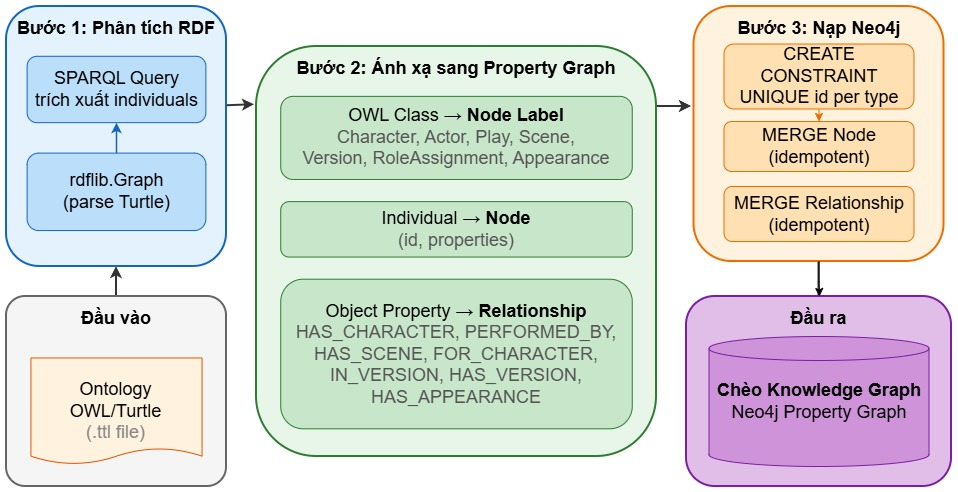
\includegraphics[width=\textwidth]{figures/c3/ontology_conversion.jpg}
  \caption{Quy trình chuyển đổi Ontology OWL~2 sang đồ thị tri thức.}
  \label{fig:ontology_conversion}
\end{figure}

\textbf{Mở rộng phân lớp nhân vật.}
Trong đồ thị cơ sở, mọi nhân vật đều mang chung nhãn \texttt{Character} và chỉ khác nhau ở giá trị thuộc tính \texttt{mainType}. Cách biểu diễn này buộc phân hệ truy xuất phải lọc theo thuộc tính tại thời điểm truy vấn, làm giảm khả năng ánh xạ câu hỏi tự nhiên sang đồ thị (vốn dựa chủ yếu vào nhãn nút) của hệ thống. Lớp \texttt{Character} do đó được mở rộng thành năm lớp con tương ứng với năm loại vai truyền thống của chèo: \texttt{DaoCharacter} (vai nữ), \texttt{KepCharacter} (vai nam), \texttt{HeCharacter} (vai hề), \texttt{MuCharacter} (nữ lớn tuổi) và \texttt{LaoCharacter} (nam lớn tuổi) (Bảng \ref{tab:schema_extension}). Mỗi nhân vật sau mở rộng mang đồng thời nhãn cha \texttt{Character} và nhãn con tương ứng - chẳng hạn Thị Kính mang nhãn \texttt{:Character} và \texttt{:DaoCharacter}. Thuộc tính \texttt{mainType} sau đó được loại bỏ vì thông tin đã chuyển sang nhãn nút; thuộc tính \texttt{subType} (Chín, Lệch, Pha, Áo dài\ldots) tiếp tục được giữ để biểu diễn phân loại chi tiết hơn trong cùng loại vai.

\textbf{Mở rộng phân loại biểu diễn.}
Lớp \texttt{Appearance} ban đầu gộp mọi loại biểu đạt -- cảm xúc, trang phục, cử chỉ -- vào cùng một loại nút, gây mơ hồ khi câu hỏi nhắm tới một thể loại cụ thể. Lớp này được phân thành ba nhóm con: \texttt{Mood} (cảm xúc nhân vật tại một lần xuất hiện, kế thừa các thuộc tính \texttt{start}/\texttt{end}/\texttt{emotion} từ \texttt{Appearance}, liên kết tới diễn viên thực hiện qua quan hệ \texttt{EXPRESS}); \texttt{Costume} (trang phục đặc trưng theo loại vai, liên kết tới diễn viên đảm nhận qua \texttt{IS\_WEAR\_BY}); và \texttt{FaceGesture} (cử chỉ khuôn mặt đại diện cho từng cảm xúc theo quy ước biểu cảm chèo) (Bảng \ref{tab:schema_extension}).

\begin{table}[ht!]
  \centering
  \caption{Các lớp con bổ sung trong đồ thị tri thức Chèo.}
  \label{tab:schema_extension}
  \renewcommand{\arraystretch}{1.3}
  \footnotesize
  \begin{tabular}{p{3.6cm} p{2.8cm} p{8.39cm}}
    \toprule
    \textbf{Lớp con} & \textbf{Lớp cha} & \textbf{Ngữ nghĩa và vai trò thiết kế} \\
    \midrule
    \texttt{DaoCharacter}
      & \texttt{Character}
      & Vai Đào - vai nữ trong vở chèo. \\[2pt]
    \texttt{KepCharacter}
      & \texttt{Character}
      & Vai Kép - vai nam trong vở chèo. \\[2pt]
    \texttt{HeCharacter}
      & \texttt{Character}
      & Vai Hề - nhân vật hài, phản biện. \\[2pt]
    \texttt{MuCharacter}
      & \texttt{Character}
      & Vai Mụ - nhân vật nữ lớn tuổi. \\[2pt]
    \texttt{LaoCharacter}
      & \texttt{Character}
      & Vai Lão - nhân vật nam lớn tuổi. \\[4pt]
    \texttt{Mood}
      & \texttt{Appearance}
      & Trạng thái cảm xúc của nhân vật tại một lần xuất hiện; gắn với
        thời gian \texttt{start}/\texttt{end} và giá trị
        \texttt{emotion} thừa kế từ \texttt{Appearance}. \\[2pt]
    \texttt{Costume}
      & \texttt{Appearance}
      & Trang phục đặc trưng theo loại vai (Đào-Chín, Hề-Áo ngắn\ldots);
        liên kết tới các diễn viên thông qua quan hệ \texttt{IS\_WEAR\_BY}. \\[2pt]
    \texttt{FaceGesture}
      & \texttt{Appearance}
      & Cử chỉ khuôn mặt đại diện cho từng loại cảm xúc theo quy ước
        biểu cảm trong nghệ thuật Chèo. \\
    \bottomrule
  \end{tabular}
\end{table}


\textbf{Mở rộng quan hệ.}
Bên cạnh phân lớp con, đồ thị tri thức được làm giàu bằng sáu quan hệ mới (Bảng~\ref{tab:relation_extension}). Hai quan hệ \texttt{EXPRESS} và \texttt{IS\_WEAR\_BY} được thiết lập ngay tại pha mở rộng schema; bốn quan hệ còn lại -- \texttt{PERFORMS}, \texttt{COLLABORATES\_WITH}, \texttt{REPRESENT}, \texttt{ARCHETYPE\_SIMILAR} -- được sinh ra qua bộ luật suy diễn (Mục~\ref{sec:retrieval_optimization}).

\begin{table}[ht!]
  \centering
  \caption{Các quan hệ bổ sung trong đồ thị tri thức Chèo.}
  \label{tab:relation_extension}
  \renewcommand{\arraystretch}{1.3}
  \footnotesize
  \begin{tabular}{p{3.6cm} p{4.4cm} p{6.79cm}}
    \toprule
    \textbf{Quan hệ} & \textbf{Domain $\to$ Range} & \textbf{Vai trò ngữ nghĩa} \\
    \midrule
    \texttt{EXPRESS}
      & \texttt{Actor} $\to$ \texttt{Mood}
      & Diễn viên biểu lộ cảm xúc qua một lần xuất hiện cụ thể. \\[2pt]
    \texttt{IS\_WEAR\_BY}
      & \texttt{Costume} $\to$ \texttt{Actor}
      & Trang phục được mặc bởi diễn viên đảm nhận vai. \\[2pt]
    \texttt{PERFORMS}
      & \texttt{Actor} $\to$ \texttt{Character}
      & Quan hệ trực tiếp diễn viên - nhân vật, rút gọn từ chuỗi qua
        \texttt{RoleAssignment}. \\[2pt]
    \texttt{COLLABORATES\_WITH}
      & \texttt{Actor} $\leftrightarrow$ \texttt{Actor}
      & Hai diễn viên cùng tham gia một phiên bản trình diễn (đối xứng). \\[2pt]
    \texttt{REPRESENT}
      & \texttt{Costume} $\to$ \texttt{Mood}
      & Trang phục thể hiện một loại cảm xúc khi co-occur thường xuyên. \\[2pt]
    \texttt{ARCHETYPE\_SIMILAR}
      & \texttt{Character} $\leftrightarrow$ \texttt{Character}
      & Hai nhân vật ở hai vở khác nhau có cùng kiểu hình kịch (đối xứng). \\
    \bottomrule
  \end{tabular}
\end{table}

\begin{figure}[!ht]
  \centering
  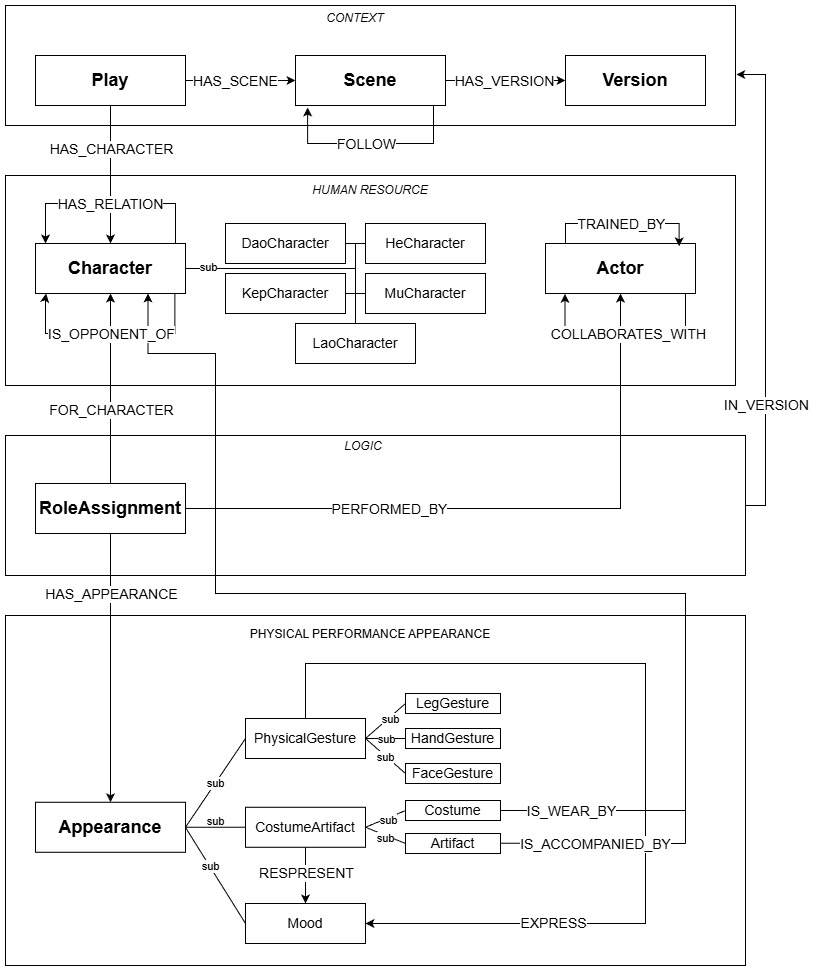
\includegraphics[width=\textwidth]{figures/c3/Ontology2.jpg}
  \caption{Lược đồ đồ thị tri thức Chèo sau mở rộng.}
  \label{fig:kg_schema}
\end{figure}

Kết quả của quá trình này chính là một đồ thị tri thức đã được mở rộng (Hình \ref{fig:kg_schema}), bảo toàn nguyên vẹn ngữ nghĩa của ontology gốc, có sự bổ sung thêm các phân lớp con và quan hệ mới để hỗ trợ trực tiếp các truy vấn đặc thù của miền nghệ thuật Chèo.

% ============================================================

\subsection{Cơ chế hỗ trợ truy xuất}
\label{sec:retrieval_optimization}

Bên cạnh lược đồ, hiệu năng truy xuất còn phụ thuộc vào hai cơ chế bổ trợ: bộ luật suy diễn xử lý quan hệ gián tiếp và chỉ mục đa mức phục vụ truy cập thực thể nhanh.

\textbf{Bộ luật suy diễn quan hệ gián tiếp.}
Đồ thị mở rộng đã lưu trữ được toàn bộ tri thức tường minh, nhưng một phần tri thức ngầm -- gồm các quan hệ chỉ hiện ra qua chuỗi liên kết nhiều bước và các quy ước nghệ thuật chưa được mã hoá -- không truy xuất được trực tiếp. Hệ thống bổ sung thêm 14 luật suy diễn được vật chất hóa lên đồ thị tại thời điểm xây dựng, chia thành ba nhóm theo chức năng. Toàn bộ luật được phát biểu hình thức bằng SWRL hoặc SPARQL CONSTRUCT và liệt kê đầy đủ tại Phụ lục~B.

\textit{Nhóm A} (gồm 4 luật A.1-A.4) đóng vai trò kiểm tra chất lượng dữ liệu một cách tự động. Trên một ontology xây dựng thủ công với hàng trăm thực thể, các vi phạm như giới tính diễn viên không khớp giới tính nhân vật hay nhân vật thiếu phân loại vai diễn rất khó được phát hiện thông qua việc duyệt thủ công. Nhóm luật này có nhiệm vụ rà soát toàn bộ đồ thị và gắn nhãn các cá thể vi phạm để yêu cầu xử lý trước khi xuất ra đồ thị tri thức hoàn chỉnh. Tiêu biểu, luật \textit{Orphaned Appearance Detection} (A.4) đã phát hiện 17 lượt Appearance tồn tại trong ontology gốc nhưng không được liên kết với bất kỳ vai diễn nào - một vấn đề chất lượng dữ liệu mà người soạn ontology không nhận ra trong quá trình xây dựng.

\textit{Nhóm B} (gồm 7 luật B.1--B.7) phục vụ mục tiêu rút gọn cấu trúc đồ thị nhằm hỗ trợ truy xuất với tốc độ nhanh hơn. Nhiều câu hỏi của người dùng đòi hỏi truy xuất các quan hệ chỉ tồn tại dưới dạng chuỗi liên kết nhiều bước trong ontology gốc, làm tăng độ phức tạp của truy vấn Cypher và đẩy cao độ trễ truy xuất. Các luật trong nhóm này tính sẵn những quan hệ phái sinh đó và lưu chúng thành các cạnh tường minh trên đồ thị. Chẳng hạn, luật \textit{Direct Performs Relation} (B.2) vật chất hoá quan hệ giữa diễn viên và nhân vật - vốn phải đi qua nút trung gian \texttt{RoleAssignment} - thành cạnh \texttt{PERFORMS} một bước, qua đó đưa độ sâu duyệt từ 3-5 bước xuống còn 1 bước cho các truy vấn tương ứng.

\textit{Nhóm C} (gồm 3 luật C.1--C.3) đảm nhận việc nhúng các tri thức nghệ thuật ngoại sinh không thể suy ra thuần tuý từ dữ liệu mà phải được lập trình theo lý thuyết chèo cổ truyền. Các quy ước hình thành qua nhiều thế hệ thực hành sân khấu được biểu diễn dưới dạng OWL Restriction hoặc cạnh suy diễn nhúng trực tiếp vào schema. Một ví dụ điển hình là luật \textit{Expected Gender per Role Type} (C.1), biểu diễn quy ước ``vai Đào và Mụ luôn là nữ, vai Kép và Lão luôn là nam'' thành ràng buộc lớp con - đảm bảo tính nhất quán ngữ nghĩa khi đồ thị được mở rộng sang các vở chèo mới.

Toàn bộ luật suy luận được thực thi sẵn ngay tại pha xây dựng đồ thị bằng mã nguồn của hệ thống, không thông qua bộ suy luận của ontology toàn cục, nhờ đó tránh được chi phí suy luận tại thời điểm truy vấn và phạm vi áp dụng các luật được kiểm soát chặt chẽ ngay từ giai đoạn thiết kế.

\textbf{Chỉ mục đa mức.}
Một câu hỏi của người dùng đi qua nhiều dạng biểu diễn của thực thể trước khi đến được nút trên đồ thị: từ tên gọi gốc xuất hiện trong câu hỏi ngôn ngữ tự nhiên, qua tên hiển thị đã được chuẩn hoá, đến định danh nội bộ duy nhất. Mỗi dạng đòi hỏi một chiến lược tra cứu riêng, vì vậy hệ thống thiết kế ba mức chỉ mục bổ trợ cho nhau (Bảng~\ref{tab:index_strategy}): chỉ mục toàn văn xử lý điểm vào -- các biến thể viết hoa hoặc viết tắt của tên riêng tiếng Việt mà người dùng có thể nhập (ví dụ ``Thị Mầu'' và ``Thị Màu'' cùng trỏ về một nhân vật); chỉ mục thuộc tính tăng tốc giai đoạn đối chiếu theo tên hiển thị đã chuẩn hoá; chỉ mục định danh phục vụ giai đoạn cuối khi câu hỏi đã được phân giải về một thực thể cụ thể. Ngoài việc khắc phục hạn chế \textit{thiếu hỗ trợ tìm kiếm văn bản} của mô hình OWL đã nêu ở Mục~\ref{sec:ontology_cheo}, sự phối hợp ba mức còn tạo nền tảng vận hành cho cơ chế Danh mục thực thể trình bày ở Mục~\ref{sec:entity_catalog} -- nơi các biến thể tên được resolve về định danh chuẩn trước khi tham gia truy vấn.

\begin{table}[ht!]
  \centering
  \caption{Chiến lược chỉ mục ba mức trên đồ thị tri thức Chèo.}
  \label{tab:index_strategy}
  \renewcommand{\arraystretch}{1.35}
  \small
  \begin{tabular}{p{3.2cm} p{4.8cm} p{6.79cm}}
    \toprule
    \textbf{Mức chỉ mục} & \textbf{Cơ chế} & \textbf{Mục tiêu và truy vấn điển hình} \\
    \midrule
    Chỉ mục định danh
      & Ràng buộc duy nhất trên định danh chuẩn của từng loại nút
      & Truy xuất $O(1)$ theo định danh; đảm bảo tính idempotent khi nạp lại dữ liệu \\[4pt]
    Chỉ mục thuộc tính
      & Chỉ mục có thứ tự trên các trường tên hiển thị của thực thể
      & Tìm kiếm $O(\log n)$ theo tên - trường xuất hiện trong phần lớn câu hỏi người dùng \\[4pt]
    Chỉ mục toàn văn
      & Chuẩn hoá hoa-thường khi đối chiếu chuỗi
      & Khớp không phân biệt hoa-thường cho tên riêng tiếng Việt với nhiều biến thể viết tắt \\
    \bottomrule
  \end{tabular}
\end{table}

\subsection{Danh mục thực thể}
\label{sec:entity_catalog}

Bên cạnh đồ thị tri thức và các chỉ mục, tầng tri thức duy trì một thành phần phụ trợ là \textbf{Danh mục thực thể} - bản trích xuất tên hiển thị của toàn bộ thực thể có trong đồ thị tri thức. Khi hệ thống khởi động, danh mục được xây dựng bằng cách quét bốn nhãn chính (\texttt{Play}, \texttt{Character}, \texttt{Actor}, \texttt{Scene}) để thu thập tên hiển thị của toàn bộ cá thể, sau đó được giữ trong bộ nhớ tiến trình để truy cập với chi phí tối thiểu.

Danh mục thực thể đảm nhận hai chức năng tại hai giai đoạn khác nhau của pipeline truy vấn. \textit{Thứ nhất}, nó đóng vai trò \textit{ràng buộc định danh} cho LLM ở giai đoạn trích xuất thực thể: prompt trích xuất chứa sẵn danh sách tên hợp lệ kèm ràng buộc \emph{chỉ chọn thực thể thuộc danh sách}, qua đó loại bỏ khả năng mô hình tạo ra tên không tồn tại trong đồ thị ngay từ bước đầu tiên - một trong những cơ chế chống ảo giác chủ chốt của hệ thống. \textit{Thứ hai}, danh mục đóng vai trò chuẩn hoá định danh trước khi truy vấn đồ thị: các biến thể viết hoa hoặc viết tắt trong câu hỏi người dùng được khớp về tên định danh chuẩn, giảm thiểu rủi ro lệch khớp do khác biệt hình thức.


